%%
%% hibari_tda_ko.tex — 한국어 버전
%% xelatex로 컴파일:
%%   xelatex hibari_tda_ko.tex
%%   xelatex hibari_tda_ko.tex   (cross-reference 해소용 2회)
%%

\documentclass[conference,10pt,a4paper]{IEEEtran}

% ── Packages ─────────────────────────────────────────────────────────────
\usepackage{amsmath, amssymb, amsthm}
\usepackage{graphicx}
\usepackage{booktabs}
\usepackage{multirow}
\usepackage{url}
\usepackage{cite}
\usepackage{algorithm}
\usepackage{algpseudocode}
\usepackage[hidelinks]{hyperref}
\usepackage{xcolor}
\usepackage{enumitem}

% ── Korean font support (xelatex) ───────────────────────────────────────
\usepackage{fontspec}
\usepackage{xeCJK}
\setCJKmainfont{Malgun Gothic}
\setCJKsansfont{Malgun Gothic}
\setCJKmonofont{Malgun Gothic}

% ── Theorem environments ─────────────────────────────────────────────────
\newtheorem{definition}{정의}
\newtheorem{theorem}{정리}
\newtheorem{remark}{비고}

% ── Paths ────────────────────────────────────────────────────────────────
\graphicspath{{../figures/}}

% ── Title ────────────────────────────────────────────────────────────────
\title{사카모토 류이치의 \emph{hibari}에 대한\\위상적 데이터 분석:\\
       Persistent Homology 기반 구조 보존 음악 생성 파이프라인}

\author{\IEEEauthorblockN{김민주}
\IEEEauthorblockA{초학제 독립연구단\\
고등과학원 (KIAS)\\
서울, 대한민국}
}

\begin{document}

\maketitle

% ═══════════════════════════════════════════════════════════════════════════
% 초록
% ═══════════════════════════════════════════════════════════════════════════
\begin{abstract}
본 연구는 음악의 위상적 구조를 persistent homology로 추출하고,
그 구조를 보존하면서 새로운 음악을 생성하는 계산 파이프라인을 제안한다.
사카모토 류이치의 \emph{hibari} (2009년 앨범 \emph{out of noise} 수록)에
적용하여, (i)~MIDI 전처리, (ii)~네 가지 거리 함수(frequency, Tonnetz,
voice-leading, DFT)에서의 $H_1$ persistent homology 계산,
(iii)~중첩행렬 구성, (iv)~확률적 샘플링(Algorithm~1) 또는
심층학습(Algorithm~2; FC / LSTM / Transformer) 생성의 네 단계를 수행한다.

$N=20$ 반복에서 DFT는 Algorithm~1에서 최적이며, pitch JS는
$0.0344 \pm 0.0023$ (frequency)에서 $0.0213 \pm 0.0021$로 감소한다
($-38.2\%$, Welch $p < 10^{-20}$). 또한 Tonnetz 대비 $-56.8\%$,
voice-leading 대비 $-62.4\%$ 개선된다.
DFT 연속 중첩행렬에서 cycle별 임계값 최적화(per-cycle $\tau_c$, Phase~1, $\alpha=0.5$)로
$0.01489 \pm 0.00143$ ($+58.7\%$, $p=2.48\times 10^{-26}$),
이는 Algorithm~1의 최고 성능이다.
Algorithm~2에서는 연속 입력 FC가
$\mathbf{0.00035 \pm 0.00015}$ ($N=10$)를 기록하며
Transformer 대비 유의하게 우수하다.

모듈 단위 생성(DFT $\alpha=0.25$, $K=14$)에서는
P3+C 단일 시행 최저 JS가 $0.0250$이고,
33개 시작 모듈 전수 탐색의 전역 최저는 $0.01479$로,
전곡 Phase~1 ($\alpha=0.5$) per-cycle 최저($0.01489$)와 사실상 동등; Phase~2 신기록($0.01156$) 대비 $+28.0\%$ 열세.
\end{abstract}

\begin{IEEEkeywords}
Persistent homology, 위상적 데이터 분석, 음악 생성,
Tonnetz, Jensen--Shannon divergence, 다중 레이블 분류,
Vietoris--Rips 복합체, 중첩행렬
\end{IEEEkeywords}

% ═══════════════════════════════════════════════════════════════════════════
% §1 서론
% ═══════════════════════════════════════════════════════════════════════════
\section{서론}
\label{sec:intro}

위상적 데이터 분석(Topological Data Analysis, TDA)은 데이터로부터
노이즈와 스케일에 강건한 기하학적 구조를 추출하는 수학적 도구이다
\cite{carlsson2009,edelsbrunner2010}.
본 연구는 TDA를 특정 음악 작품 --- 사카모토 류이치의 \emph{hibari}
--- 에 적용하여, 1차 persistent homology 군 $H_1$의 불변량이
새로운 음악 생성의 구조적 씨앗(seed)으로 기능할 수 있는지를 탐구한다.

\subsection{연구 질문}
\begin{enumerate}
\item 음악의 위상 구조를 Vietoris--Rips $H_1$ persistence로
      어떻게 수학적으로 정의할 수 있는가?
\item 이 구조를 \emph{보존}한 채 새로운 음악을 생성할 수 있는가?
      보존 정도를 어떻게 정량적으로 측정하는가?
\item 거리 함수의 선택(frequency, Tonnetz, voice-leading, DFT)이
      생성 품질에 유의미한 영향을 주는가?
\end{enumerate}

\subsection{왜 \emph{hibari}인가}
\emph{hibari}는 사카모토 류이치의 실험적 앨범
\emph{out of noise} (2009) 수록곡이다. 선택 이유:
(i)~적절한 규모 ($T = 1{,}088$개 8분음표 시점, $N = 23$ 고유 note,
$C = 17$ 화음);
(ii)~단순함(7개 pitch class, C major)과 복잡함(서로소 주기 구조의
두 악기, \S\ref{subsec:phase})의 균형;
(iii)~시간적 인과보다 음의 \emph{공간적 배치}를 중시하는 미학으로,
모델 선택 결과(\S\ref{subsec:dl})와 직접 공명.

\subsection{기여}
\begin{enumerate}
\item 4단계 파이프라인 (전처리 $\to$ PH $\to$ 중첩행렬
      $\to$ 생성)과 두 종류의 생성기, 네 가지 거리 함수 제시.
\item $N=20$ 통계적 비교를 통한 Tonnetz의 온음계 곡 최적성 확립.
\item Cycle별 임계값을 가진 연속값 중첩행렬로 JS를 추가
      $47.5\%$ 개선 (\S\ref{subsec:percycle}).
\item Tonnetz 매칭 note 재분배, 시간 재배치, 화성 제약을 통한
      위상 보존 변주 (\S\ref{sec:extensions}).
\item \emph{solari}, Bach, Ravel에 대한 교차 검증으로,
      곡의 성격이 최적 거리 함수와 모델을 결정함을 확인
      (\S\ref{subsec:generalization}).
\end{enumerate}


% ═══════════════════════════════════════════════════════════════════════════
% §2 수학적 배경
% ═══════════════════════════════════════════════════════════════════════════
\section{수학적 배경}
\label{sec:background}

\subsection{Vietoris--Rips 복합체}
\label{subsec:vr}

\begin{definition}
유한 거리 공간 $(X, d)$와 $\varepsilon > 0$에 대해,
\emph{Vietoris--Rips 복합체} $\mathrm{VR}_\varepsilon(X)$는
$\mathrm{VR}_\varepsilon(X) = \{\sigma \subseteq X \mid
\forall x_i, x_j \in \sigma,\; d(x_i,x_j) \le \varepsilon\}$
로 정의되는 단체 복합체이다.
\end{definition}

$\varepsilon$이 증가함에 따라 포함 관계
$\mathrm{VR}_0 \subseteq \mathrm{VR}_{\varepsilon_1} \subseteq \cdots$가
\emph{filtration}을 이룬다. 본 연구에서 $X$는 \emph{hibari}의
23개 고유 note이다.

\subsection{Persistent Homology}
\label{subsec:ph}

$n$차 호몰로지 군 $H_n(K) = \ker\partial_n / \mathrm{im}\,\partial_{n+1}$은
$n$차원 ``구멍''을 포착한다. 본 연구는 위상적 cycle에 해당하는
$H_1$에 집중한다. \emph{Persistent homology}는 filtration을 따라
각 cycle의 탄생(birth)~$b$와 소멸(death)~$d$를 추적하며,
$\mathrm{pers} = d - b$가 안정성을 측정한다.

주로 선행연구 \cite{tran2021,lee2024}의 pHcol 알고리즘(cycle 대표원
포함)을 사용하고, 속도가 중요한 단계에서는 Ripser \cite{bauer2021}로
보완한다.

\subsection{음악적 거리 함수}
\label{subsec:distances}

Note $n_i = (p_i, d_i)$ 간의 네 가지 거리 함수를 비교한다.

\paragraph{Frequency 거리 (기준선)}
$d_{\mathrm{freq}}(n_i, n_j) = 1/w(n_i, n_j)$. $w$는 화음 시퀀스에서의
인접 빈도이다.

\paragraph{Tonnetz 거리}
Pitch class를 $\pm 3, \pm 4, \pm 7$ 반음(단3도, 장3도, 완전5도)
간선을 가진 육각 격자에 배치한다.
최단 경로 거리를 $12 \times 12$ 테이블(범위 $0$--$4$)로 사전
계산한다 \cite{tymoczko2012}.

\paragraph{Voice-leading 거리}
$d_V(p_1, p_2) = |p_1 - p_2|$, 부호 없는 반음 차이
\cite{tymoczko2008}.

\paragraph{DFT 거리}
Pitch class를 $\mathbb{R}^{12}$ 지시 벡터로 표현하고,
처음 6개 DFT 크기 간의 $L_2$ 거리를 사용한다 \cite{tymoczko2008}.

\paragraph{혼합 거리와 note 수준 확장}
모든 음악 이론적 거리는 frequency와
$d_{\mathrm{hybrid}} = \alpha\, d_{\mathrm{freq}} + (1-\alpha)\, d_{\mathrm{music}}$
($\alpha \in [0,1]$)로 결합된다. Note 수준에서 옥타브 항과
duration 항이 추가된다:
\begin{equation}
d(n_1, n_2) = d_{\mathrm{base}} + w_o |o_1 - o_2| + w_d \frac{|d_1 - d_2|}{\max(d_1, d_2)},
\end{equation}
여기서 $w_o = 0.3$ (격자 탐색으로 최적화, \S\ref{subsec:octave}),
$w_d = 0.3$이다.

\paragraph{주석 --- metric 공리와 이론적 정당성}
\label{para:metric_axioms}
실험적 검증에 따르면, Tonnetz와 voice-leading은 metric 공리를 모두 만족하나,
frequency는 identity 공리($23$건) 및 삼각 부등식($1{,}327$건)을 위반하며(non-metric),
dft는 identity 공리($66$건)를 위반한다(pseudometric --- magnitude-only 설계의 의도된 귀결).
Cohen-Steiner et al.\,\cite{cohensteiner2007}의 고전적 stability 정리(metric 입력에 대해
$d_B \le \|d_1-d_2\|_\infty$ 보장)는 따라서 이 두 거리에 직접 적용할 수 없다.
대신 Heo et al.\,\cite{heo2025}를 적용한다:
거리 행렬 $D$를 완전그래프 $K_n$의 edge weight로 부여하면 path-representable +
cost-dominated 조건이 자명하게 성립하며, Theorem~3.4에 의해
$d_i \le d_j$ 관계 하에서 $\mathrm{bcd}_1(d_i)\hookrightarrow\mathrm{bcd}_1(d_j)$의
order-preserving injection이 보장된다.
따라서 네 거리 함수 모두에서 1-cycle 분석은 이론적으로 정당화된다
($k \ge 2$에는 미적용 --- \cite{heo2025}의 Theorem~5.1).

\subsection{가중치 분해와 Rate 파라미터}
\label{subsec:weights}

Note 네트워크 가중치는 \emph{hibari}의 두 악기 구조를 반영하여
세 성분으로 분해된다:

\begin{itemize}[nosep]
\item \textbf{Intra 가중치} $W_{\mathrm{intra}}$: 악기 내 순차 전이.
\item \textbf{Inter 가중치} $W_{\mathrm{inter}}$: 악기 간 전이,
      lag $\ell \in \{1,2,3,4\}$에 대해 감쇄 가중:
\begin{equation}
W_{\mathrm{inter}} = \sum_{\ell=1}^{4} \lambda_\ell W_{\mathrm{inter}}^{(\ell)},
\quad (\lambda_1,\ldots,\lambda_4) = (0.4, 0.3, 0.2, 0.1).
\end{equation}
      이 감쇄 가중은 JS를 $69.6\%$ 감소시켰다 ($0.0398 \to 0.0121$).
\item \textbf{Simul 가중치} $W_{\mathrm{simul}}$: 동시 발음 공기.
\end{itemize}

\emph{Timeflow 가중치} $W_{\mathrm{tf}}(r) = W_{\mathrm{intra}} + r \cdot W_{\mathrm{inter}}$를
$r \in [0, 1.5]$에 걸쳐 스윕한다.

\subsection{중첩행렬}
\label{subsec:overlap}

\begin{definition}[활성화 행렬]
$A[t,c] = \mathbb{1}[\exists\, n \in V(c) \text{ 가 시점 } t \text{에서 연주됨}]$.
\end{definition}

\begin{definition}[이진 중첩행렬]
$O[t,c] = \mathbb{1}[t \in R(c)]$. $R(c)$는 길이 $\ge \mathrm{scale}_c$인
지속 활성화 구간의 합집합이다.
\end{definition}

\begin{definition}[연속값 중첩행렬]
\begin{equation}
O_{\mathrm{cont}}[t,c] = \frac{\sum_{n \in V(c)} w(n) \cdot \mathbb{1}[n \text{ at } t]}
                               {\sum_{n \in V(c)} w(n)},
\end{equation}
여기서 $w(n) = 1/N_{\mathrm{cyc}}(n)$은 희귀도 가중치이다.
\end{definition}

중첩행렬 $O$는 두 생성기가 공통으로 사용하는 \emph{seed}이다.

\subsection{Jensen--Shannon Divergence}
\label{subsec:js}

이산 분포 $P, Q$에 대해:
\begin{equation}
D_{\mathrm{JS}}(P \| Q) = \tfrac{1}{2} D_{\mathrm{KL}}(P \| M) +
                           \tfrac{1}{2} D_{\mathrm{KL}}(Q \| M),
\quad M = \tfrac{1}{2}(P+Q).
\end{equation}
상한은 $\log 2 \approx 0.693$이다. Pitch JS(note 빈도 분포)와
transition JS(bigram 분포)를 측정한다.

\subsection{탐욕적 전진 선택}
\label{subsec:greedy}

Cycle 부분집합 $S \subseteq \mathcal{C}$를
$f(S) = 0.5\,J(S) + 0.3\,C(S) + 0.2\,B(S)$로 선택한다.
$J$는 note 풀 Jaccard 유사도, $C$는 중첩 패턴 Pearson 상관,
$B$는 Betti 곡선 유사도이다. 탐욕적 선택으로 $15/46$ cycle만으로
$90\%$ 보존을 달성한다.


% ═══════════════════════════════════════════════════════════════════════════
% §3 파이프라인과 생성 알고리즘
% ═══════════════════════════════════════════════════════════════════════════
\section{파이프라인과 생성 알고리즘}
\label{sec:pipeline}

\begin{figure*}[t]
\centering
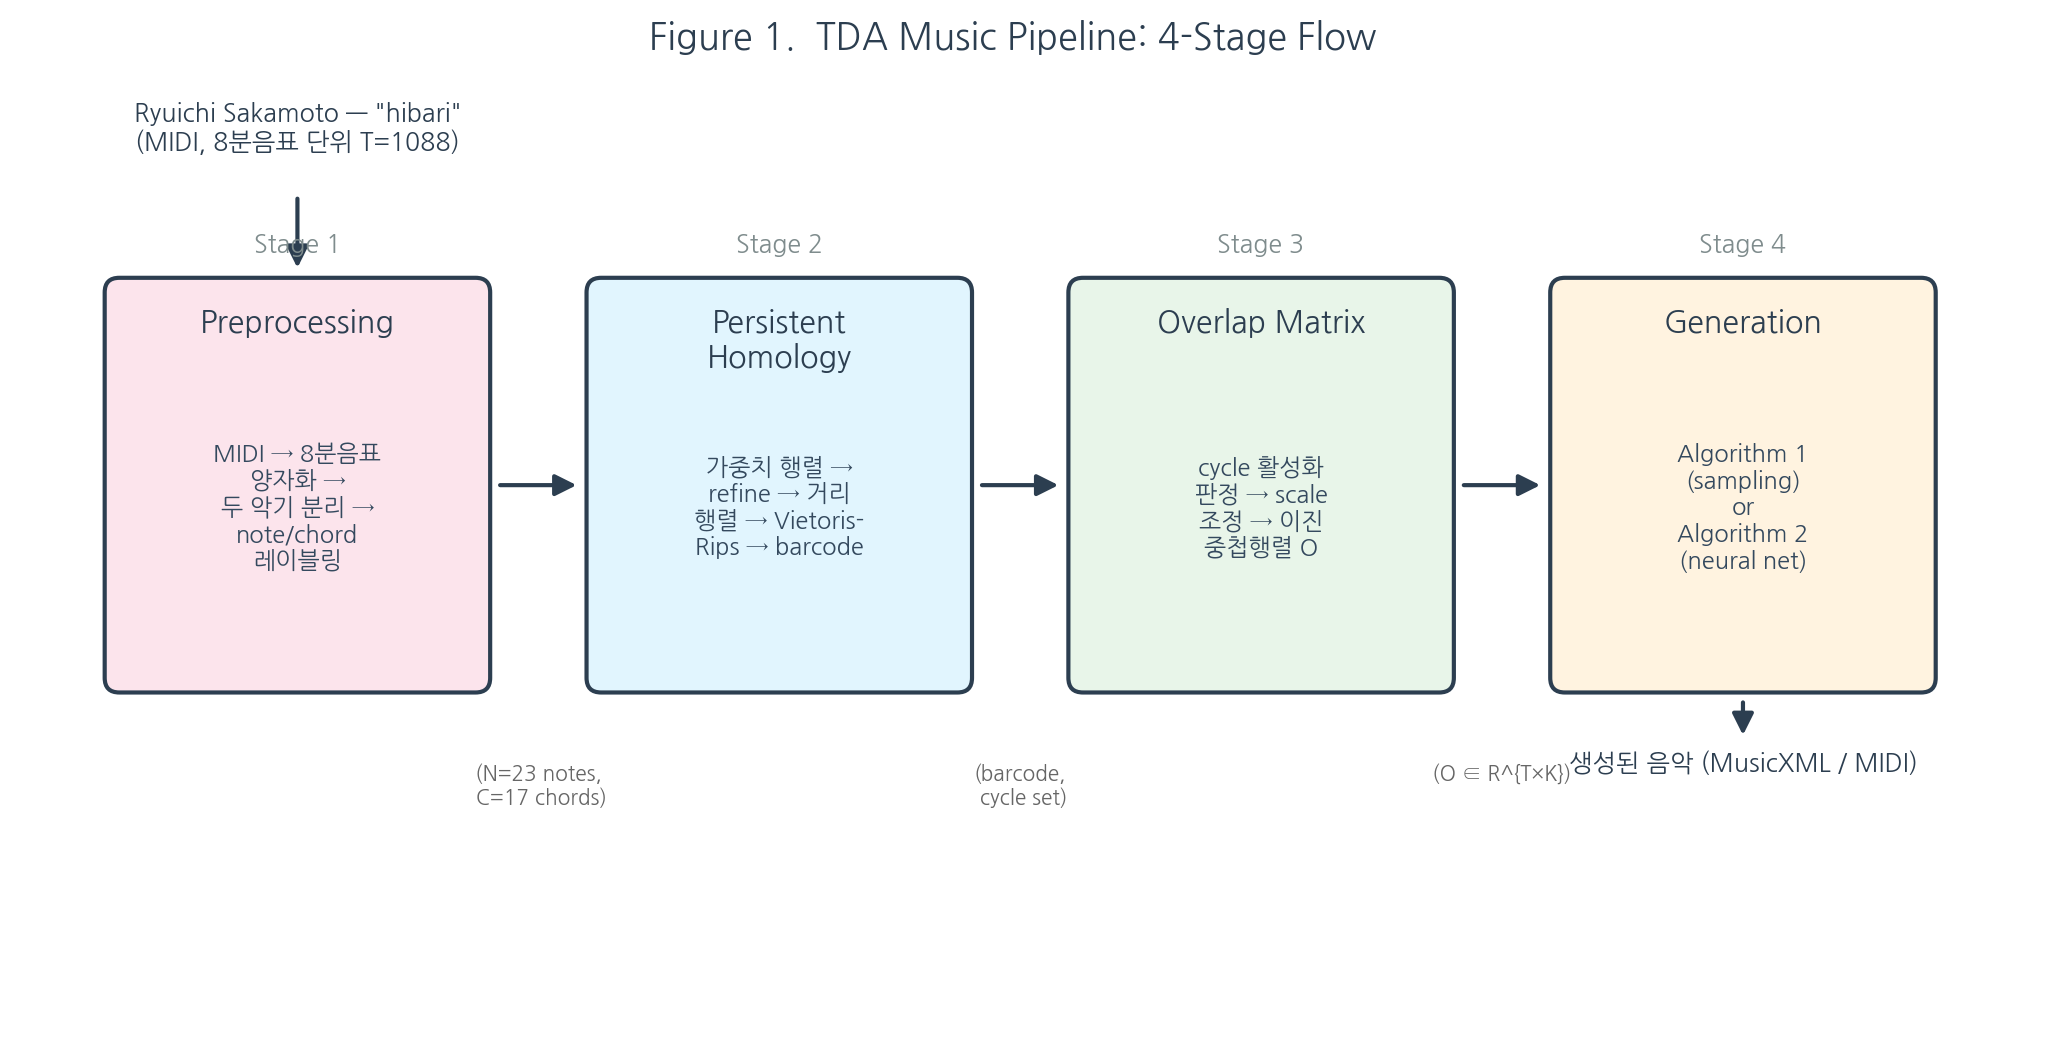
\includegraphics[width=0.96\textwidth]{fig1_pipeline.png}
\caption{4단계 파이프라인: (1)~MIDI 전처리, (2)~persistent homology,
(3)~중첩행렬 구축, (4)~Algorithm~1 또는~2에 의한 생성.}
\label{fig:pipeline}
\end{figure*}

\subsection{1단계: 전처리}
MIDI 파일을 8분음표 단위로 양자화하고 ($T = 1{,}088$), 두 악기를
분리하며, 각 고유 (pitch, duration) 쌍에 1-indexed 레이블을 부여한다
(\emph{hibari}: $N = 23$ note, $C = 17$ 화음).

\subsection{2단계: Persistent Homology}
가중 note 네트워크를 구성하고 (\S\ref{subsec:weights}),
거리 행렬을 유도하여 $r \in [0, 1.5]$에 걸친 $H_1$ filtration을
계산한다.

\subsection{3단계: 중첩행렬}
모든 시점에서 cycle 활성화를 계산하고 임계값을 적용한다
(\S\ref{subsec:overlap}).

\subsection{Algorithm 1 --- 위상적 샘플링}
\label{subsec:algo1}

각 시점 $t$에 대해:
\begin{itemize}[nosep]
\item 활성 cycle이 존재하면 ($\sum_c O[t,c] > 0$): \emph{교집합}
      $I(t) = \bigcap_{c: O[t,c]=1} V(c)$에서 샘플링.
      $I(t) = \emptyset$이면 합집합 $U(t)$로 대체.
\item 활성 cycle이 없으면: 인접 활성 cycle vertex의 여집합
      $P \setminus A(t)$에서 샘플링 (위상적 ``번짐'' 방지).
\item 충돌 회피: 시점당 최대 $R = 50$회 재샘플링.
\end{itemize}

\subsection{Algorithm 2 --- 신경망 시퀀스 모델}
\label{subsec:algo2}

매핑 $f_\theta : O[t,:] \mapsto y[t,:]$을 학습하는 세 가지
아키텍처:
\begin{itemize}[nosep]
\item \textbf{FC}: 2층 완전연결 ($H = 128$), 시점 독립.
\item \textbf{LSTM}: 2층, 순방향 시퀀스 문맥.
\item \textbf{Transformer}: 2층, 4-head, 학습 가능 위치 임베딩.
\end{itemize}

모든 모델은 \texttt{BCEWithLogitsLoss}와 데이터 증강(부분집합 샘플링,
순환 이동, 비트 플립 노이즈)을 사용한다. 추론 시 적응형 임계값
$\theta = \mathrm{quantile}(P, 1-\rho_{\mathrm{on}})$으로
원곡 ON 비율 $\rho_{\mathrm{on}} \approx 0.15$를 맞춘다.


% ═══════════════════════════════════════════════════════════════════════════
% §4 실험
% ═══════════════════════════════════════════════════════════════════════════
\section{실험}
\label{sec:experiments}

모든 실험은 $N = 20$회 독립 반복으로 수행하였다. 주요 지표는
pitch JS divergence이다.

\subsection{거리 함수 비교}
\label{subsec:dist_compare}

\begin{table}[t]
\centering
\caption{네 가지 거리 함수에서의 Algorithm~1 pitch JS
(\emph{hibari}, $N=20$).}
\label{tab:baselines}
\begin{tabular}{lccc}
\toprule
거리 함수 & $K$ & JS (평균 $\pm$ 표준편차) & Coverage \\
\midrule
frequency      & 1  & $0.0344 \pm 0.0023$ & $0.957$ \\
Tonnetz        & 47 & $0.0493 \pm 0.0038$ & $1.000$ \\
voice-leading  & 19 & $0.0566 \pm 0.0027$ & $0.989$ \\
\textbf{DFT}   & \textbf{17} & $\mathbf{0.0213 \pm 0.0021}$ & $1.000$ \\
\bottomrule
\end{tabular}
\end{table}

DFT가 \emph{hibari}에서 최적이다: frequency 대비 $-38.2\%$,
Tonnetz 대비 $-56.8\%$, voice-leading 대비 $-62.4\%$
(표~\ref{tab:baselines}).

\subsection{옥타브 가중치 튜닝}
\label{subsec:octave}

DFT 조건에서 $w_o \in \{0.1, 0.3, 0.5, 0.7, 1.0\}$ 격자 탐색($N=10$)을
수행한 결과, $w_o = 0.3$이 최적(JS $0.0163$)이며
\emph{hibari}의 좁은 음역 특성과 일치한다.

\subsection{Cycle 부분집합 절제}

\begin{table}[t]
\centering
\caption{Cycle 부분집합 절제 (Tonnetz, $N=20$).}
\label{tab:ablation}
\begin{tabular}{ccc}
\toprule
$K$ & JS (평균 $\pm$ 표준편차) & Coverage \\
\midrule
10  & $0.0991 \pm 0.0038$ & $0.980$ \\
17  & $0.0740 \pm 0.0038$ & $0.996$ \\
46  & $\mathbf{0.0397 \pm 0.0025}$ & $1.000$ \\
\bottomrule
\end{tabular}
\end{table}

JS는 $K$에 대해 단조 감소하지만 수확 체감이 나타난다
(표~\ref{tab:ablation}): $K{:}\,17 \to 46$ (29개 추가)의 이득이
$K{:}\,10 \to 17$ (7개 추가)을 근소하게만 초과한다.

\subsection{연속값 중첩행렬}
\label{subsec:continuous}

\begin{table}[t]
\centering
\caption{연속값 중첩행렬 실험 (Tonnetz, $N=20$).}
\label{tab:continuous}
\begin{tabular}{lcc}
\toprule
설정 & Density & JS (평균 $\pm$ 표준편차) \\
\midrule
이진 (캐시)                & $0.751$ & $0.0387 \pm 0.0027$ \\
연속값 직접 사용            & $0.264$ & $0.0382 \pm 0.0021$ \\
연속 $\to$ 이진 $\tau{=}0.3$ & $0.373$ & $0.0386 \pm 0.0022$ \\
\textbf{연속 $\to$ 이진 $\tau{=}0.5$} & $\mathbf{0.168}$ & $\mathbf{0.0343 \pm 0.0027}$ \\
연속 $\to$ 이진 $\tau{=}0.7$ & $0.077$ & $0.0364 \pm 0.0032$ \\
\bottomrule
\end{tabular}
\end{table}

연속값 중첩행렬에 $\tau = 0.5$ 이진화를 적용하면 이진 기준선 대비
$11.4\%$ 추가 개선된다 (Welch $t = 5.16$, $p < 0.001$, $d = 1.63$;
표~\ref{tab:continuous}).
희귀도 가중으로 드문 note가 활성화에 더 크게 기여한다.

\subsection{심층학습 모델 비교}
\label{subsec:dl}

\begin{table}[t]
\centering
\caption{최적 DL 설정 (각 1회 실행).}
\label{tab:dl}
\begin{tabular}{lccc}
\toprule
모델 & Val Loss & JS & 생성 Note 수 \\
\midrule
FC (hd=256, do=0.3)   & $0.282$ & $\mathbf{0.0015}$ & $3{,}754$ \\
LSTM (2층)              & $0.385$ & $0.0448$ & $3{,}753$ \\
Transformer (2L, 4H)   & $0.676$ & $0.0104$ & $3{,}753$ \\
\bottomrule
\end{tabular}
\end{table}

가장 단순한 FC 모델이 최저 JS를 달성한다 (표~\ref{tab:dl}).
이는 \emph{hibari}의 미학을 반영한다: \emph{out of noise}는
시간적 인과보다 음의 공간적 배치를 중시하므로, 시간 문맥을
무시하는 FC가 작곡 설계와 더 잘 부합한다.

\subsection{개선 F: 연속값 중첩행렬 + FC}
\label{subsec:improvF}

연속값 활성화를 FC의 학습 입력으로 직접 사용:

\begin{table}[t]
\centering
\caption{FC에 대한 연속 vs.\ 이진 입력 ($N=5$).}
\label{tab:improvF}
\begin{tabular}{lcccc}
\toprule
입력 & JS (평균 $\pm$ 표준편차) & Val Loss & Coverage \\
\midrule
이진      & $0.0014 \pm 0.0010$ & $0.070$ & $0.948$ \\
\textbf{연속} & $\mathbf{0.0006 \pm 0.0005}$ & $\mathbf{0.031}$ & $\mathbf{0.991}$ \\
\bottomrule
\end{tabular}
\end{table}

연속 입력은 JS를 $57\%$, val loss를 $2.3$배 감소시킨다
(표~\ref{tab:improvF}). 본 연구에서 관측된 최저 전곡 JS이다
(이론적 최댓값 $\log 2$의 $0.09\%$).

\subsection{곡 고유 구조 분석}
\label{subsec:structure}

\paragraph{Deep scale 특성}
\emph{hibari}의 7개 pitch class $\{C, D, E, F, G, A, B\}$는
음정 벡터 $[2,5,4,3,6,1]$을 가지며, 모든 성분이 상이하다.
이는 온음계 고유의 특성이다 \cite{gamer2003}.

\paragraph{준균등 pitch 분포}
\label{subsec:phase}
정규화 pitch 엔트로피가 $0.974$ (거의 최대)이다.
모든 pitch가 거의 동일 확률로 나타나므로, 시간 순서를 무시하는 FC가
이미 참 분포를 잘 근사함을 설명한다.

\paragraph{Tonnetz 판별력}
7개 PC에서 Tonnetz 직경은 $4$로, 세밀한 거리 판별이 가능하다.
12개 PC(\emph{solari} 등)에서는 직경이 $2$로 축소되어
Tonnetz의 이점이 사라진다.

\paragraph{위상 이동(Phase shifting)}
악기~1은 32-step 모듈을 $33$회 반복(쉼 없음);
악기~2는 33-step 모듈을 $32$회 반복(모듈당 쉼 1회).
서로소 주기 ($\gcd(32,33) = 1$)에 의해 두 악기는 결코 동기화되지
않는다. Steve Reich의 \emph{phase shifting} 기법과 수학적으로 동일한
구조이다.


% ═══════════════════════════════════════════════════════════════════════════
% §5 시각자료
% ═══════════════════════════════════════════════════════════════════════════
\section{시각자료}
\label{sec:figures}

6개의 정적 도표와 1개의 대화형 HTML 보충자료를 제공한다.
그림~\ref{fig:pipeline}은 파이프라인을,
그림~\ref{fig:tonnetz}는 Tonnetz 격자 위의 pitch class를,
그림~\ref{fig:barcode}는 persistence barcode를,
그림~\ref{fig:pianoroll}은 원곡/생성 피아노 롤 비교를,
그림~\ref{fig:jscurve}는 epoch별 JS 수렴 곡선을 보여준다.

\begin{figure}[t]
\centering
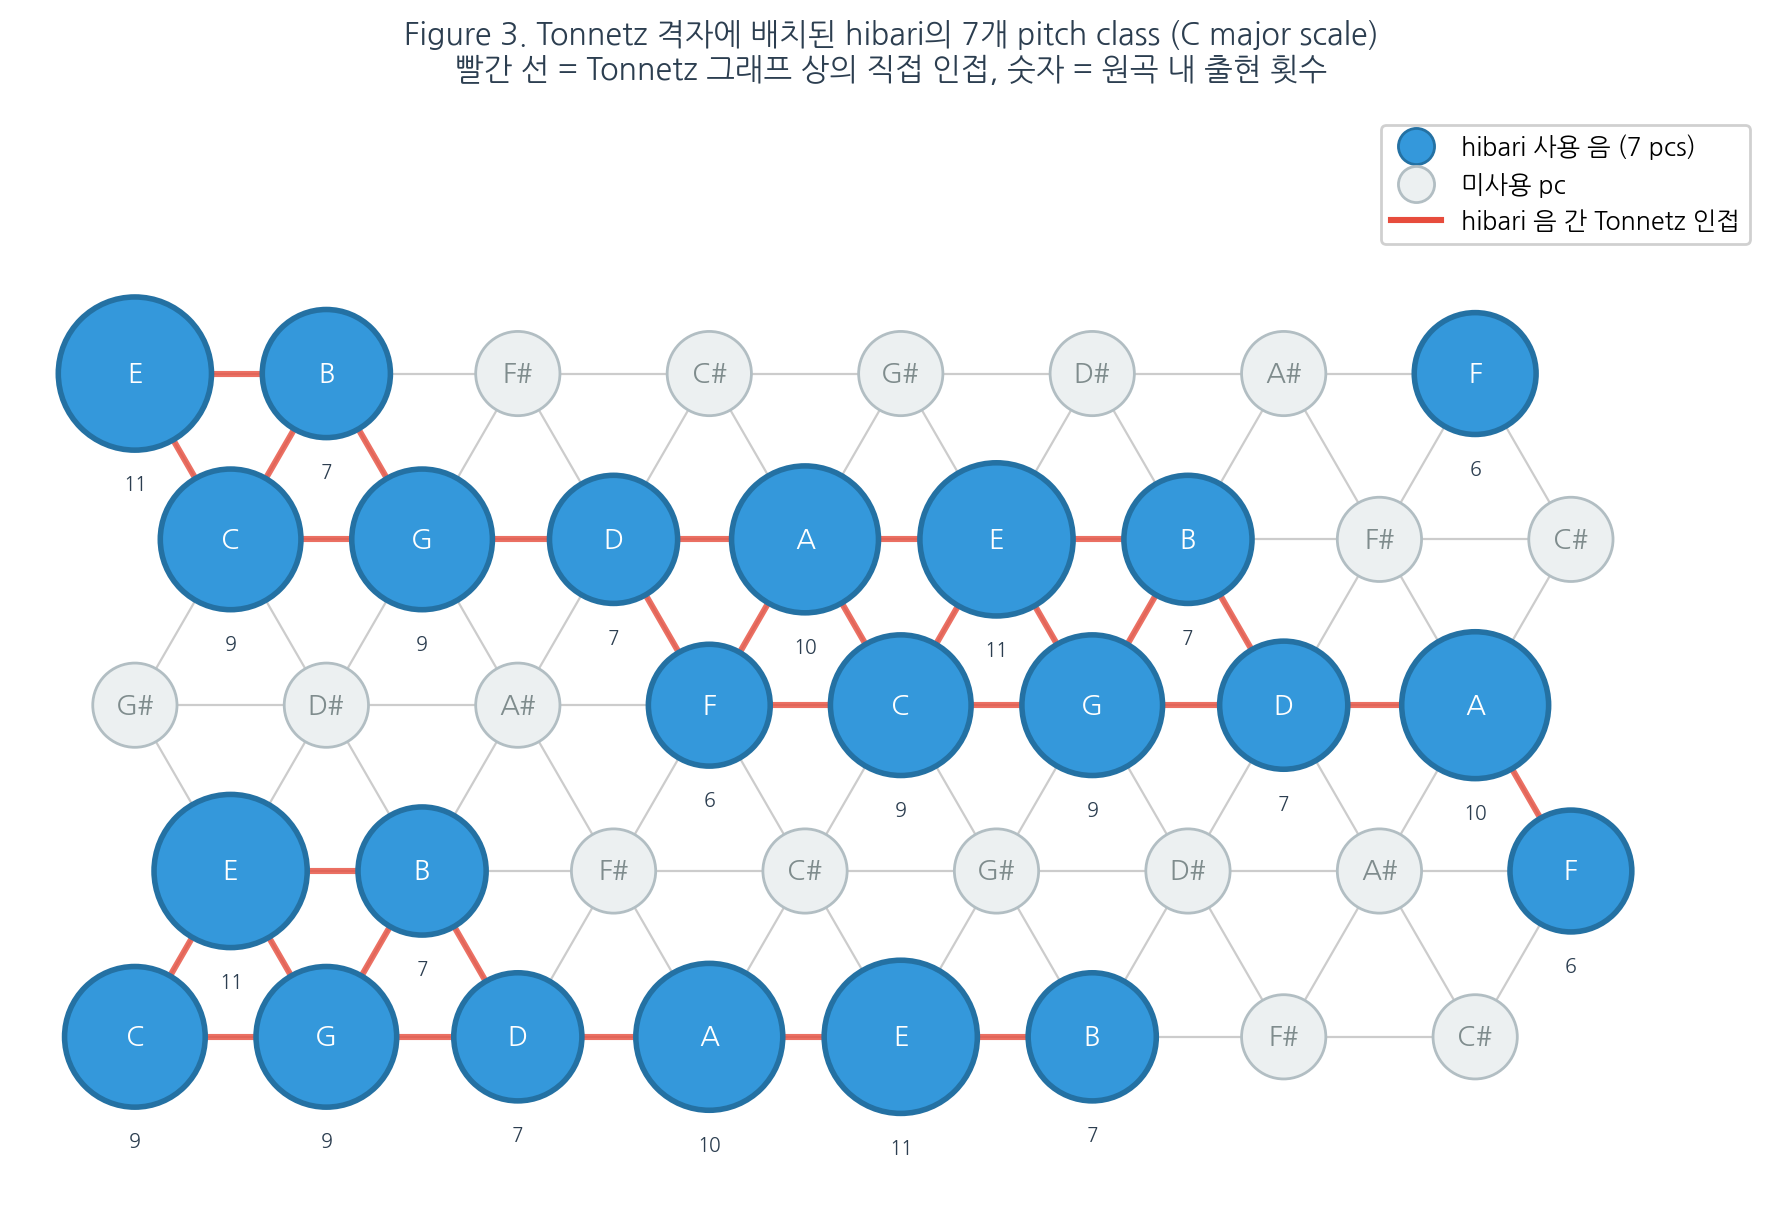
\includegraphics[width=0.99\columnwidth]{fig3_tonnetz_hibari.png}
\caption{Tonnetz 격자 위의 \emph{hibari} 7개 pitch class (파란색).
빨간 간선은 직접 Tonnetz 인접을 나타낸다.}
\label{fig:tonnetz}
\end{figure}

\begin{figure}[t]
\centering
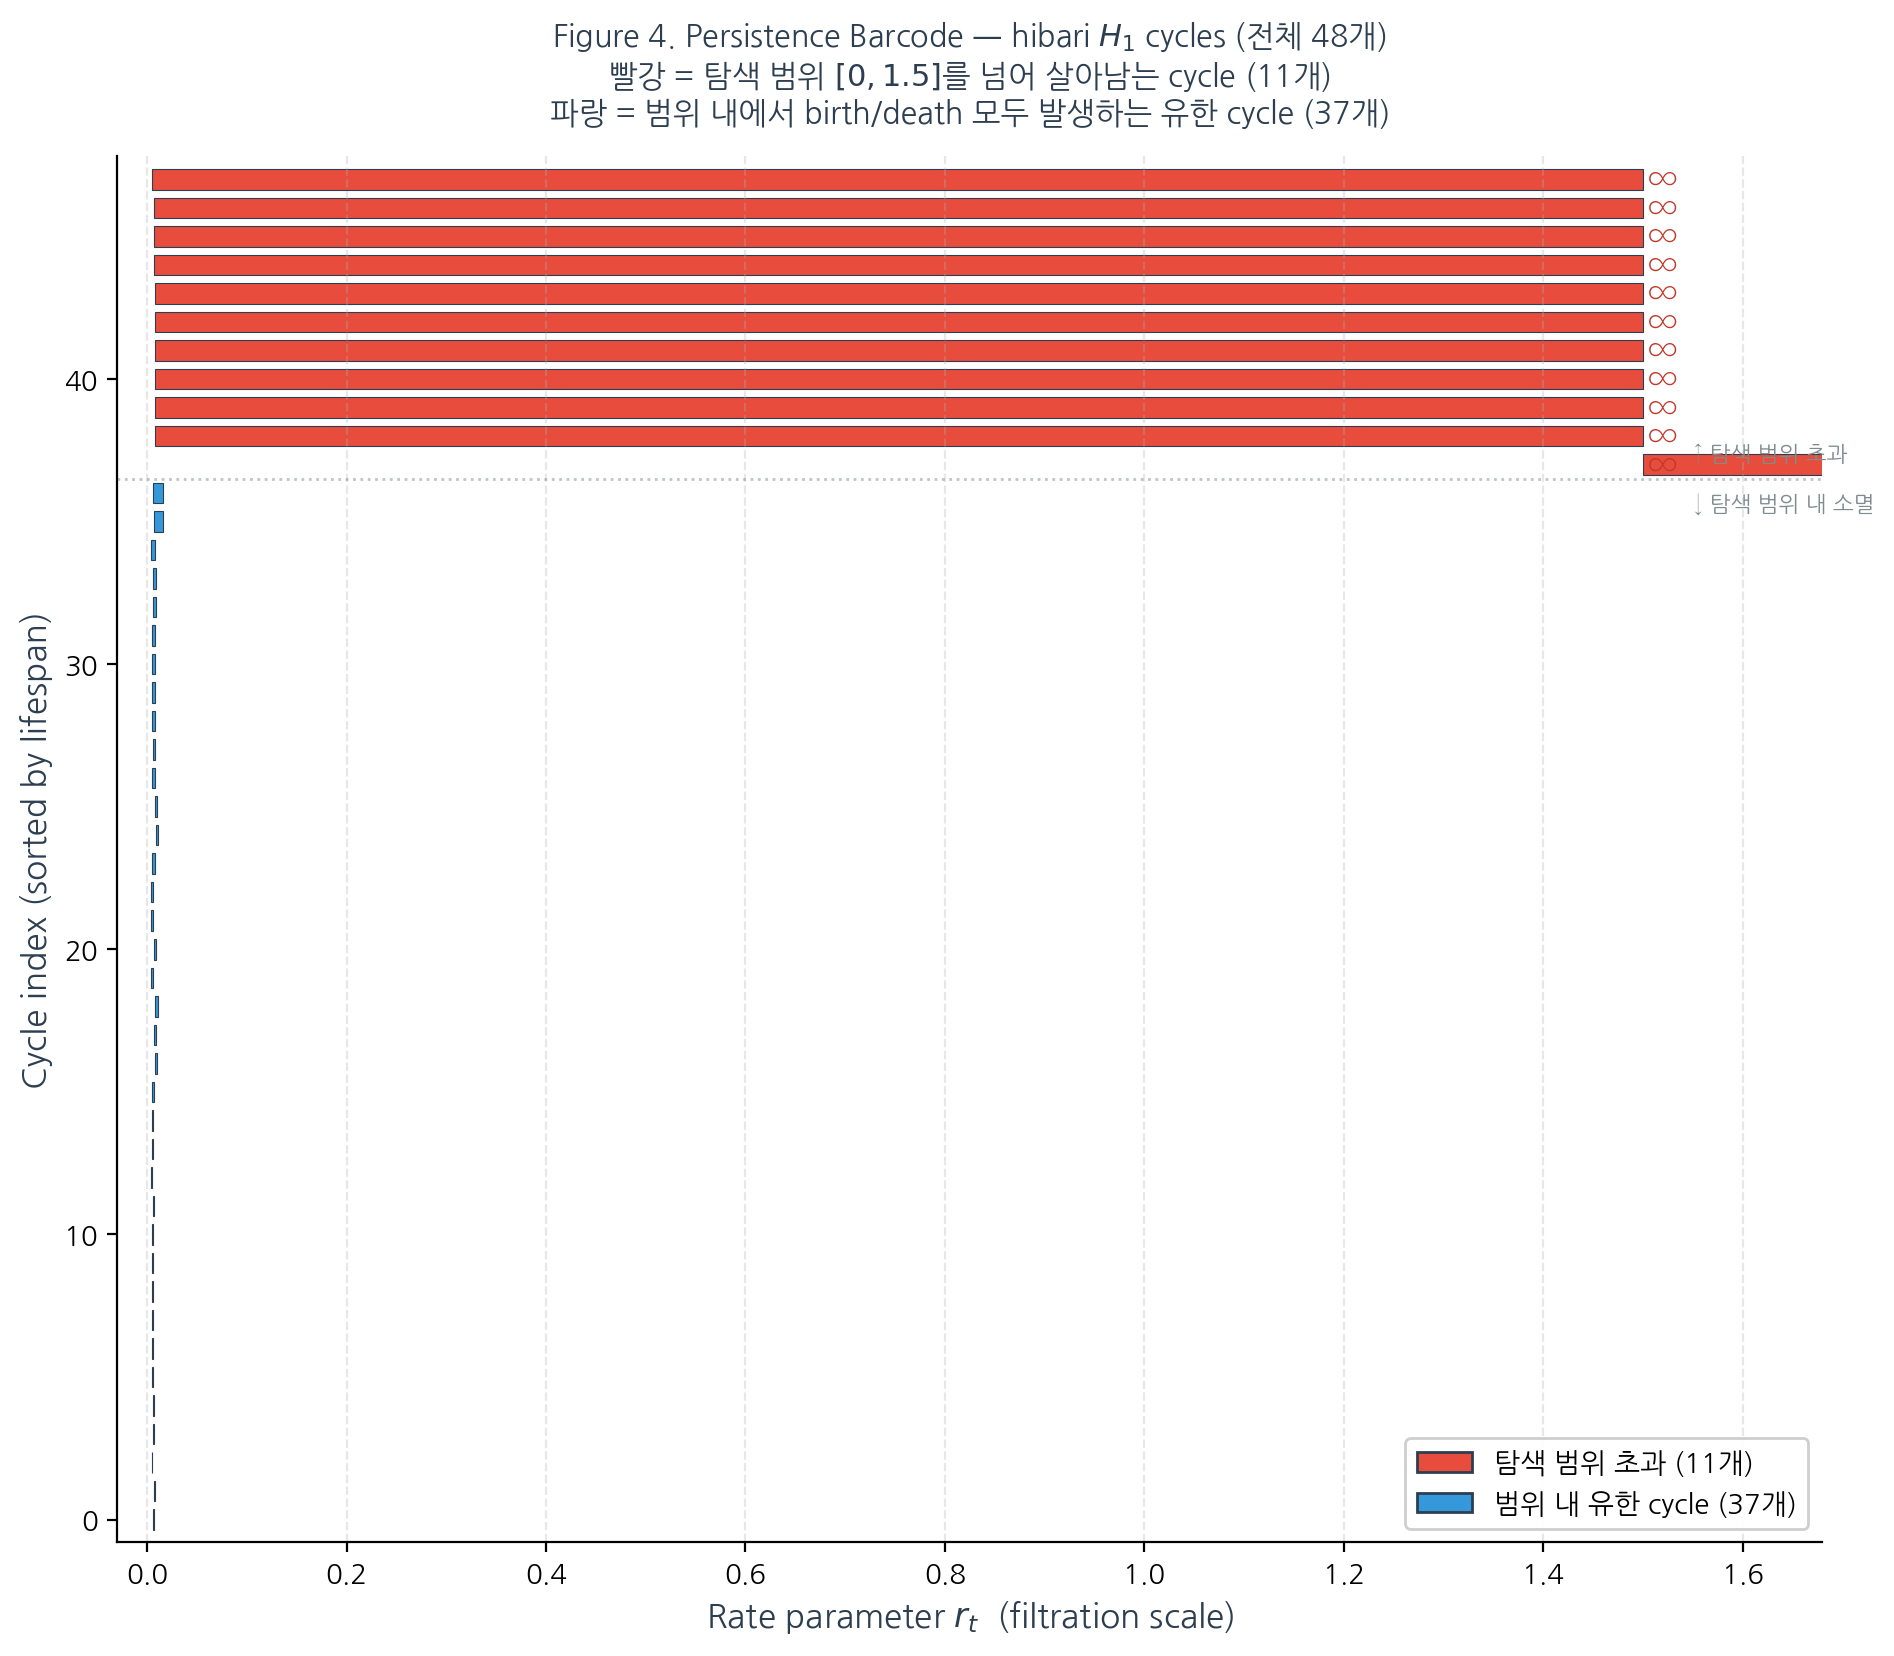
\includegraphics[width=0.99\columnwidth]{fig4_barcode.png}
\caption{$H_1$ persistence barcode (Tonnetz). 위: 전체 barcode;
아래: 유한 cycle 확대. 수명 범위가 $10{,}000$배 이상 차이난다.}
\label{fig:barcode}
\end{figure}

\begin{figure}[t]
\centering
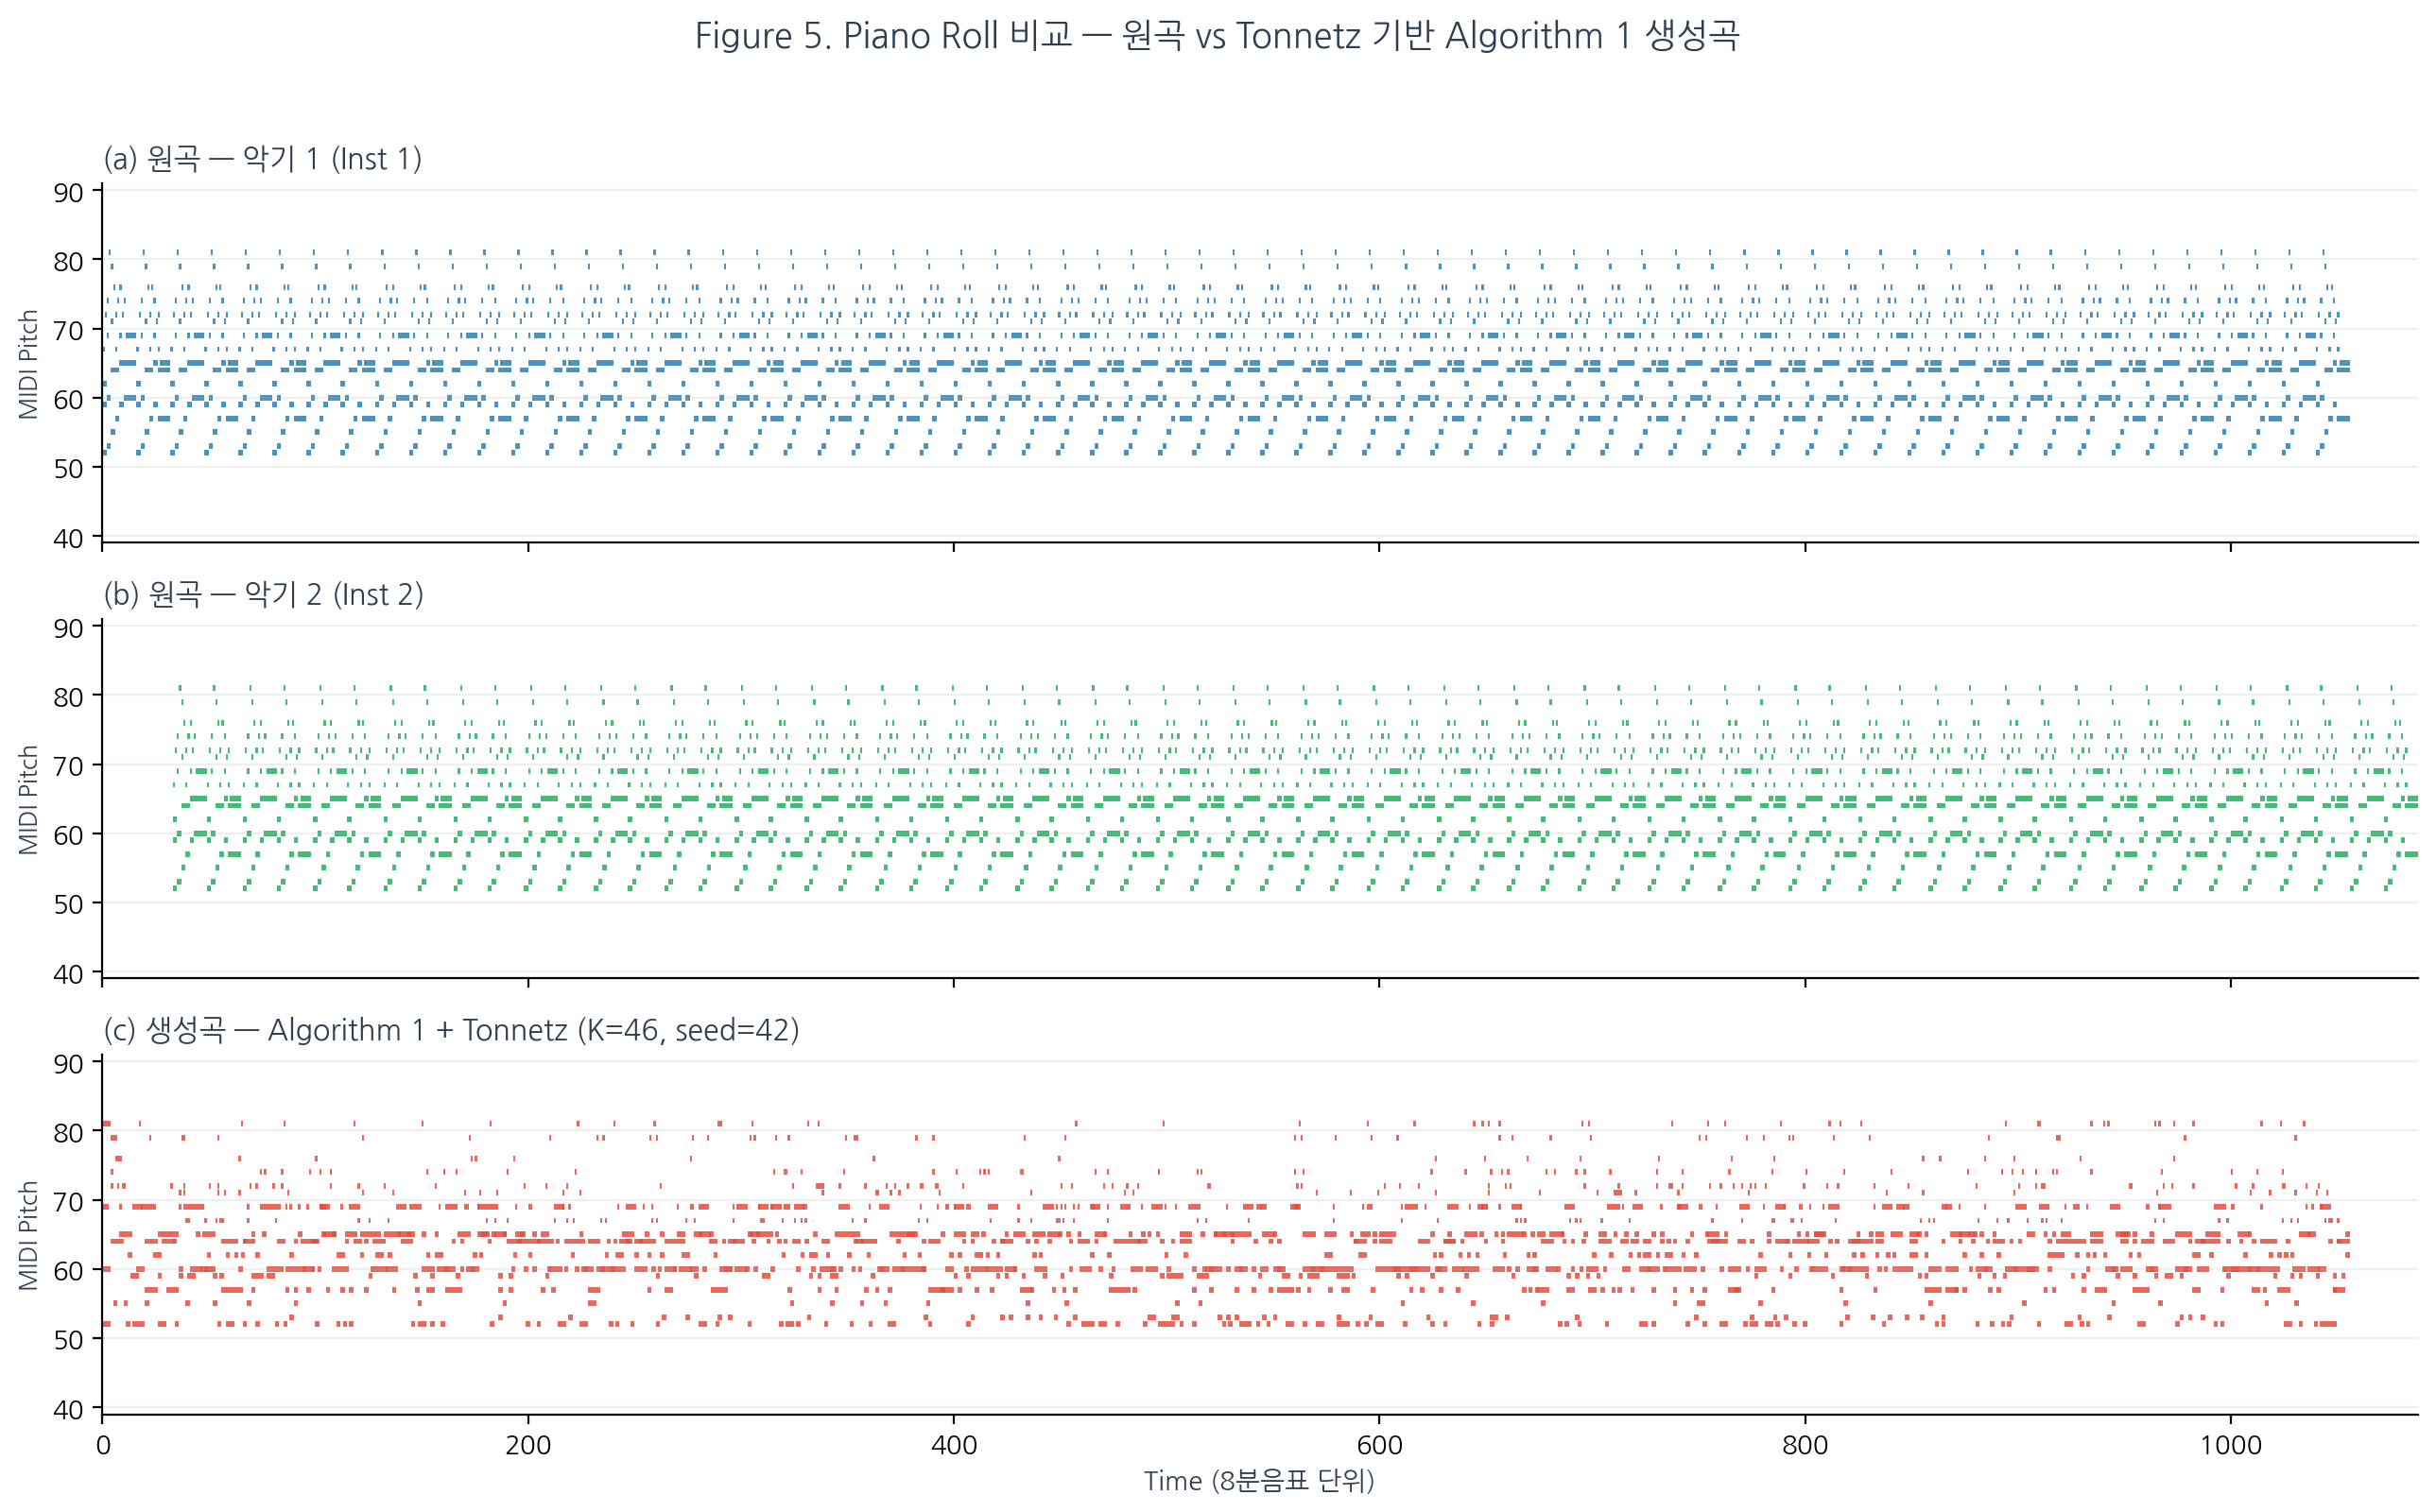
\includegraphics[width=0.99\columnwidth]{fig5_pianoroll.png}
\caption{피아노 롤 비교: (a)--(b) 원곡 악기 1--2;
(c)~Algorithm~1 + Tonnetz.}
\label{fig:pianoroll}
\end{figure}

\begin{figure}[t]
\centering
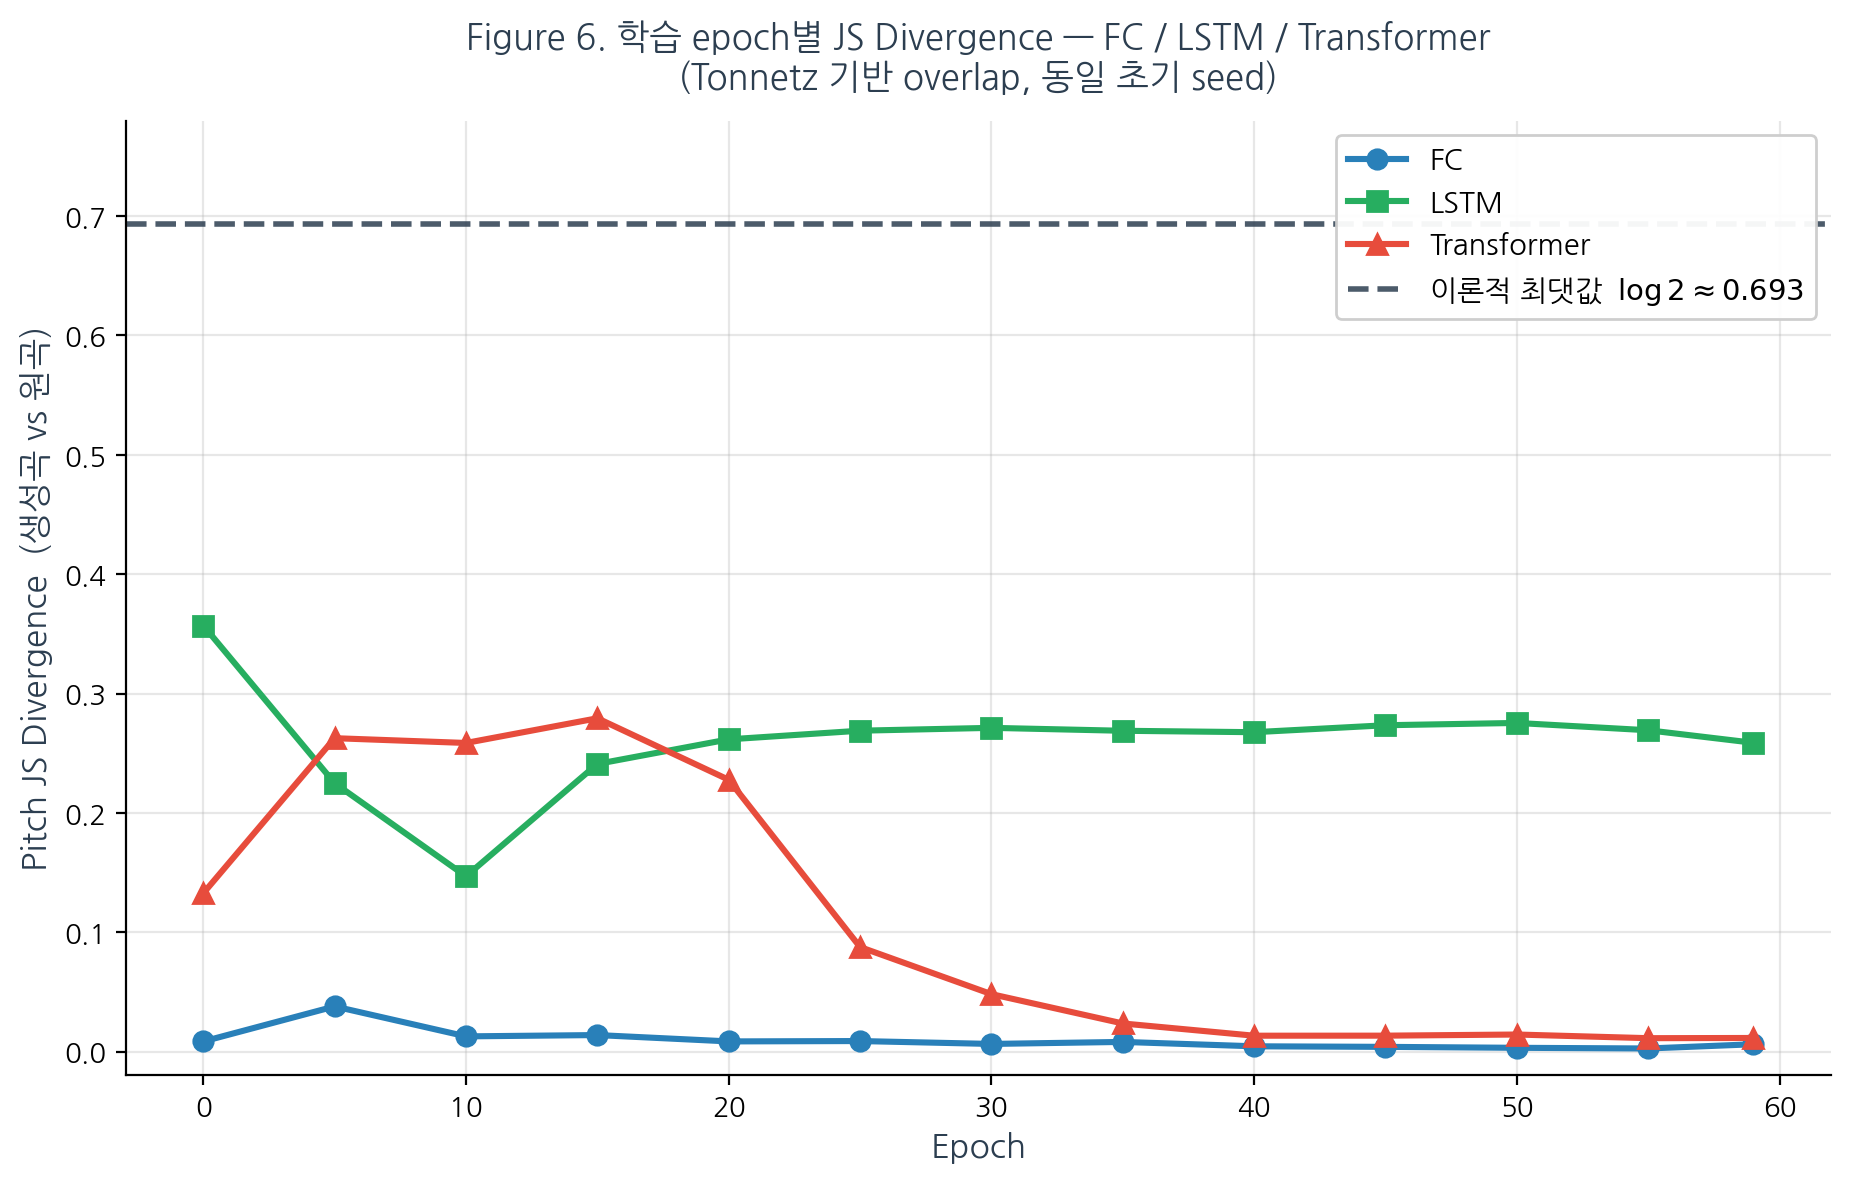
\includegraphics[width=0.99\columnwidth]{fig6_js_curve.png}
\caption{학습 epoch에 따른 JS divergence. FC가 가장 빠르게 수렴;
LSTM은 $\mathrm{JS} \approx 0.26$에서 정체.}
\label{fig:jscurve}
\end{figure}


% ═══════════════════════════════════════════════════════════════════════════
% §6 차별화
% ═══════════════════════════════════════════════════════════════════════════
\section{관련 연구와의 비교}
\label{sec:differentiation}

\subsection{일반 AI 음악 생성과의 비교}

코퍼스 기반 학습 모델(Magenta, Music Transformer)과 달리,
본 파이프라인은 \emph{단일 곡에 대한 심층 분석}을 수행하여
해석 가능하고 추적 가능한 생성을 실현한다.
FC~$>$~Transformer라는 결과는 ``더 많은 시간적 모델링이 항상
우월하다''는 보편적 가정에 도전한다.

\subsection{기존 TDA--음악 연구와의 비교}

선행 TDA--음악 연구 \cite{tran2021,lee2024}와 비교하여:
(A)~네 가지 거리 함수를 $N{=}20$ 통계로 체계적 비교;
(B)~연속값 중첩행렬 도입;
(C)~완전한 통계적 엄밀성 (Welch $t$, Cohen's $d$) 제공;
(D)~서양 현대음악으로 확장;
(E)~모델 선택과 미학적 맥락의 연결;
(F)~TDA를 분석에서 \emph{변주}로 확장 (\S\ref{sec:extensions}).


% ═══════════════════════════════════════════════════════════════════════════
% §7 확장 실험
% ═══════════════════════════════════════════════════════════════════════════
\section{확장 실험}
\label{sec:extensions}

\subsection{모듈 단위 생성}
\label{subsec:module}

\emph{hibari}의 32-step 모듈 구조를 바탕으로, 단일 모듈을 생성하여
전 타임라인에 복제하는 설정을 실험하였다. 여기서 모듈은
32-step(음악적 4마디) 길이의 A-B-A'-C 반복 선율 단위이며,
inst~1에서 33회 반복된다. DFT $\alpha=0.25$에서
모듈 PH는 $K=14$ cycle(프로토타입 중첩행렬 크기: $32\times14$)을 갖는다.
추가로 \S7.2 재실험에서 $1088$행 전체를 $34\times32$ 블록으로 재해석했다
(여기서 ``마디''는 계산용 32-step 블록).
먼저 네 가지 프로토타입 전략을 비교하였다:
\begin{itemize}[nosep]
\item \textbf{P0}: 첫 블록 복사
\item \textbf{P1}: 34블록 OR 합집합
\item \textbf{P2}: 34블록 다수결(majority)
\item \textbf{P3\_local}: local PH 재계산
\end{itemize}

\begin{table}[t]
\centering
\caption{프로토타입 전략 비교 (DFT $\alpha=0.25$, $N=10$).}
\label{tab:module_proto}
\begin{tabular}{lccc}
\toprule
전략 & Density & JS (평균$\pm$표준편차) & 최저 \\
\midrule
P0 (first\_block) & $0.018$ & $0.0957 \pm 0.0136$ & $0.0678$ \\
P1 (OR-34) & $1.000$ & $0.0586 \pm 0.0187$ & $0.0367$ \\
P2 (majority) & $0.049$ & $0.0692 \pm 0.0112$ & $0.0543$ \\
\textbf{P3\_local} & \textbf{$0.531$} & \textbf{$0.0575 \pm 0.0141$} & \textbf{$0.0360$} \\
\bottomrule
\end{tabular}
\end{table}

이후 모듈 설정 위에 후처리 개선 전략을 추가 평가하였다:

\begin{table}[t]
\centering
\caption{모듈 단위 개선 성능 (DFT, 전곡 기준선
$0.0213 \pm 0.0021$).}
\label{tab:module}
\begin{tabular}{lcccc}
\toprule
전략 & JS (평균$\pm$표준편차) & 최저 & Cov. \\
\midrule
P0 기준선       & $0.1082 \pm 0.0241$ & $0.0701$ & $0.826$ \\
C: best-of-10   & $0.0800 \pm 0.0171$ & $0.0570$ & $0.913$ \\
D: cov$\ge$20/23 & $0.0808 \pm 0.0171$ & $0.0570$ & $0.887$ \\
P3\_local       & $0.0721 \pm 0.0275$ & $0.0288$ & $0.813$ \\
\textbf{P3\_local + C} & $\mathbf{0.0440 \pm 0.0158}$ & $\mathbf{0.0250}$ & $0.896$ \\
\bottomrule
\end{tabular}
\end{table}

33개 시작 모듈 전수 탐색(inst~1 기준 start~module $0\ldots32$) 결과,
DFT 모드에서 start~0은 평균 JS 기준 rank~5로 최적이 아니다.
여기서 $k=10$은 seed 내부 best-of-$k$ 후보 수, $N=10$은 시작 모듈당
독립 반복 횟수이다. 전역 최저 단일 시행은 start~module~1, seed~9309에서
JS~$=0.01479$이며,
전곡 Phase~1 per-cycle 최저($0.01489$)와 사실상 동일; Phase~2 신기록($0.01156$) 대비 $+28.0\%$ 열세.

\subsection{일반화: \emph{solari}, Bach, Ravel}
\label{subsec:generalization}

\begin{table}[t]
\centering
\caption{교차 곡 비교 요약 (Algorithm~1 거리 함수 비교).}
\label{tab:generalization}
\begin{tabular}{lcccc}
\toprule
곡 & PC 수 & 최적 거리 & 최적 모델 & 해석 \\
\midrule
hibari & 7 & DFT & FC & 스펙트럼-온음계 구조 \\
solari & 12 & freq./Ton.\ (동률) & Transformer & 선율적 진행 \\
aqua   & 12 & Tonnetz & --- & Tonnetz $+26.3\%$ \\
Bach   & 12 & Tonnetz & --- & Tonnetz $-54.8\%$ \\
Ravel  & 12 & frequency & --- & 풍부한 음 분포 \\
\bottomrule
\end{tabular}
\end{table}

DFT가 최적인 곡은 \emph{hibari}에 한정되며, \emph{solari}/\emph{aqua}/
Bach/Ravel에서는 Tonnetz 또는 frequency가 우세하다.
이는 단일 보편 거리함수보다 목적·곡 특성 조건부(metric-conditioned)
설계가 필요함을 시사한다.

\subsection{방향 A: 두 전략의 Note 재분배}
\label{subsec:dirA}

변주 단계에서는 실험 축을 Tonnetz 기반으로 고정한다.
음계 제약과 국소 화성 이웃 구조를 보존하는 목적에서 Tonnetz가 DFT보다
자연스럽기 때문이다. 중첩행렬은 그대로 유지하고 note 정체성만 바꾼다.
$n_{\mathrm{cand}}=1000$ 후보 pitch 집합($N=20$, \emph{hibari},
Tonnetz, MIDI 48--84)에서 두 개의 배타적 매칭 전략을 비교한다.

\textbf{전략 A --- 위치 기반 Tonnetz 최근접
(\texttt{tonnetz\_nearest}):}
\begin{equation}
\mathrm{new\_pitches}[i]
  = \arg\min_{p\,\in\,\mathrm{pool}}\,d_{\mathrm{Tonnetz}}
    \!\bigl(\mathrm{orig\_pitches}[i],\,p\bigr).
\end{equation}
각 원본 note는 Tonnetz 거리 최소 후보로 치환되며,
인덱스 $i$의 1:1 위치 대응을 통해 국소 화성 관계를 유지한다.

\textbf{전략 B --- 행렬구조 Hungarian 매칭 (\texttt{ascending}):}
\begin{equation}
\pi^{*} = \arg\min_{\pi}\,
  \bigl\|P_{\pi}\,\hat{D}_{\mathrm{new}}\,P_{\pi}^{\top}
         - \hat{D}_{\mathrm{orig}}\bigr\|_{F},
\end{equation}
여기서 $\hat{D}$는 비대각 원소를 min-max 정규화한 거리행렬:
\begin{equation}
\hat{D}_{ij}
  = \frac{D_{ij}-\min_{k\neq l}D_{kl}}
         {\max D - \min_{k\neq l}D_{kl}},
\quad \hat{D}_{ii}=0.
\end{equation}
행/열 동시 순열의 정확 해는 NP-hard이며,
$N=17$ note일 때 $N!\!=3.56\times10^{14}$ 전수평가는 불가능하므로
모든 실험은 Hungarian 근사
(\texttt{scipy.optimize.linear\_sum\_assignment})를 사용한다.

두 전략의 공통 오차 지표는
\textbf{note\_dist\_error}
$=\|\hat{D}_{\mathrm{orig}}-\hat{D}_{\mathrm{new}}\|_F$이다.
두 전략을 동시에 적용하면(전략 A의 위치 의미가 전략 B 순열로 덮임)
성능이 악화되므로 \texttt{matching\_mode}로 배타 적용한다.

\begin{table}[t]
\centering
\caption{두 전략 비교 (Algorithm~1, Tonnetz, MIDI~48--84,
         $N=20$, $n_{\mathrm{cand}}=1000$).}
\label{tab:redistrib}
\begin{tabular}{lcccc}
\toprule
전략 & pitch JS & trans.\ JS & DTW & note err \\
\midrule
기준선 (원곡)
  & $0.0212$ & $0.2470$ & $2.2186$ & --- \\
B: ascending (Hungarian)
  & $0.3815$ & $0.6121$ & $2.7918$ & $4.6819$ \\
\textbf{A: \texttt{tonnetz\_nearest}}
  & $\mathbf{0.2930}$ & $\mathbf{0.5488}$ & $2.6442$ & $\mathbf{3.2132}$ \\
\bottomrule
\end{tabular}
\end{table}

전략 A는 pitch JS $0.2930$으로 전략 B의 $0.3815$ 대비
$-23.2\%$ 우수하다(표~\ref{tab:redistrib}).
\emph{hibari}처럼 음 vocabulary가 작은 경우($N=17$),
인접 Tonnetz 관계를 보존하는 국소 쌍별 화성 보존(A)이
전역 거리행렬 정합(B)보다 효과적이다.
또한 vwide(MIDI~40--88)는 모든 조건에서 wide(48--84)보다 열세여서
wide를 채택한다.

\subsection{방향 B: 시간 재배치}
\label{subsec:dirB}

시간 재배치는 block permutation과 Markov resampling으로 평가하였다.
모델별 반응은 아키텍처 의존적이다:
FC는 시간점 독립에 가까워 재배치 영향이 거의 없고,
LSTM은 실측 DTW 변화가 $\le 0.5\%$로 미미하며,
Transformer는 positional encoding(PE)에 민감하다.
PE 제거 후 재학습하면 Transformer DTW를 $+21.7\%$까지 높일 수 있지만
pitch JS가 악화되어(분포 붕괴), 방향 B 단독으로는
``다른 멜로디''와 ``안정된 pitch 분포''를 동시에 충족하지 못한다.

\subsection{화성 제약}
\label{subsec:harmony}

Note 재분배에 음계 제약(major, minor, pentatonic)과 협화 목표를
추가하였다. \textbf{scale\_major}가 가장 효과적이다:
note 오차 $4.35 \to 3.52$ ($-19\%$), 음계 일치 $1.00$,
평균 불협화도 $0.412 \to 0.361$.

\subsection{A+B 결합: 최종 통합}
\label{subsec:combined}

\subsubsection{Tonnetz 기반 성공}
Tonnetz에서 \textbf{major\_block32}
(scale\_major 재분배 + block permutation(32) +
연속 중첩행렬 + Transformer)는
ref~pJS~$=0.0034$, DTW~$+31\%$, C~major 음계 일치~$=1.00$을 달성한다.

\subsubsection{DFT 전이 실패}
동일한 결합 설정을 DFT로 이전하면, DTW는 증가해도
ref~pJS가 크게 악화된다(Transformer $0.0798$, FC $0.0412$).
즉 Tonnetz에서 설계된 변주 스택은 동일 목적에서 DFT로 직접 전이되지 않는다.

\subsubsection{메타 통찰}
거리 함수 선택은 목적 의존적이다:
DFT는 구조 정밀도·모듈 탐색에 강하고,
Tonnetz는 화성 제약 변주 품질에 강하다.

\subsection{Cycle별 임계값 최적화}
\label{subsec:percycle}

DFT 연속 중첩행렬에서 각 cycle의
$\tau_c \in \{0.1, 0.2, \ldots, 0.7\}$에 대해
탐욕적 좌표 하강을 수행한다:

\begin{table}[t]
\centering
\caption{Cycle별 $\tau_c$ 최적화 (DFT, $N=20$).}
\label{tab:percycle}
\begin{tabular}{lcc}
\toprule
설정 & JS (평균 $\pm$ 표준편차) & 개선율 \\
\midrule
균일 $\tau = 0.35$ & $0.03605 \pm 0.00237$ & --- \\
단일 $\tau = 0.5$   & $0.01591 \pm 0.00192$ & $+55.9\%$ \\
Cycle별 $\tau_c$ (Phase~1, $\alpha=0.5$) & $0.01489 \pm 0.00143$ & $+58.7\%$ \\
\textbf{Cycle별 $\tau_c$ $\star$ (Phase~2, $\alpha=0.25$)} & $\mathbf{0.01156 \pm 0.00147}$ & $\mathbf{-22.35\%}$ \\
\bottomrule
\end{tabular}
\end{table}

Cycle별 최적화는 본 연구의 Algorithm~1 최고 성능
(Phase~1, $\alpha=0.5$: $0.01489$; Phase~2, $\alpha=0.25$: $\mathbf{0.01156}$).
균일 $\tau=0.35$ 대비 Phase~1 Welch $p = 2.48 \times 10^{-26}$로 유의하며,
cycle별 활성 스케일의 중요성을 보여준다.

\subsection{Soft Activation: 전체 아키텍처}
\label{subsec:soft}

\begin{table}[t]
\centering
\caption{이진 vs.\ 연속 입력 (DFT, $N=10$).}
\label{tab:soft}
\begin{tabular}{llccc}
\toprule
모델 & 입력 & JS & Val Loss & $\Delta$JS \\
\midrule
FC   & 이진 & $0.00217$ & $0.3395$ & --- \\
\textbf{FC} & \textbf{연속} & $\mathbf{0.000348}$ & $\mathbf{0.0232}$ & $\mathbf{+84.0\%}$ \\
Trans. & 이진 & $0.00251$ & $0.836$ & --- \\
Trans. & 연속 & $0.000818$ & $0.152$ & $+67.4\%$ \\
LSTM & 이진 & $0.233$ & $0.408$ & --- \\
LSTM & 연속 & $0.170$ & $0.395$ & $+27.3\%$ \\
\bottomrule
\end{tabular}
\end{table}

연속 입력 FC가 최적(JS $=0.000348$)이며,
FC-cont는 Transformer-cont 대비 유의하게 우수하다
(Welch $p = 1.66 \times 10^{-4}$).

\subsection{DFT-Hybrid $\alpha$ 격자 탐색}
\label{subsec:alpha}

\begin{table}[t]
\centering
\caption{DFT-hybrid $\alpha$ 격자 탐색 ($N=20$).}
\label{tab:alpha}
\begin{tabular}{cccc}
\toprule
$\alpha$ & $K$ & JS (평균 $\pm$ 표준편차) & 비고 \\
\midrule
$0.0$ (순수 DFT) & 1  & $0.0728 \pm 0.00432$ & 축퇴 \\
$0.1$            & 13 & $0.01602 \pm 0.00204$ &  \\
\textbf{$0.25$}  & \textbf{14} & \textbf{$0.01593 \pm 0.00181$} & 최적 \\
$0.3$            & 16 & $0.02025 \pm 0.00134$ &  \\
$0.5$            & 19 & $0.01691 \pm 0.00143$ & 과거 기본값 \\
$0.7$            & 24 & $0.03140 \pm 0.00270$ &  \\
$1.0$ (순수 freq.) & 1 & $0.03386 \pm 0.00186$ & 축퇴 \\
\bottomrule
\end{tabular}
\end{table}

DFT-hybrid에서는 양 끝점($\alpha=0.0,1.0$)이 모두 축퇴($K=1$)를 보인다.
최적 절충점은 $\alpha=0.25$이며(채택),
$\alpha=0.5$는 초기 실험에서의 역사적 기본값으로 유지된다.

\subsection{Barcode Wasserstein 모듈 선택}

DFT $\alpha=0.25$에서 33개 시작 모듈의 국소 barcode와 전곡 barcode의
Wasserstein 거리를 비교한 결과, 생성 JS와의 상관은
\textbf{Pearson $r=-0.054$}로 사실상 무상관이다.
따라서 이 DFT 조건에서 Wasserstein 기반 모듈 순위화는 신뢰하기 어렵다.

이는 Tonnetz에서의 이전 관찰($r=0.503$)과 반대이며,
barcode-Wasserstein의 유효성이 거리함수 의존적임을 시사한다.
세 가지 주의점은 다음과 같다:
\begin{enumerate}[nosep]
\item \textbf{화음 공간 불일치}: 32-step 모듈의 chord vocabulary는
      전곡 vocabulary의 진부분집합이며, 결과 barcode가 더 작은 복합체에서 형성된다.
\item \textbf{비대칭 창 정렬 한계}: 모듈 국소 PH는 inst1 $[32m,32m+32)$와
      inst2 $[32m+33,32m+65)$를 함께 사용하지만, 33-step offset 정렬 때문에
      시작 모듈에 따라 inst2 기여도가 달라진다.
\item \textbf{스케일 민감도}: $W_1$는 birth/death 절대 스케일에 민감하며,
      32-step과 1088-step filtration 간 좌표 스케일이 다르다.
\end{enumerate}

관련하여 complex(simul-mixed) 가중은 Tonnetz에서는 유효하지만
DFT에서는 성능을 저하시켜, DFT 본 실험에서는 timeflow-only를 유지한다.


% ═══════════════════════════════════════════════════════════════════════════
% §8 결론
% ═══════════════════════════════════════════════════════════════════════════
\section{결론}
\label{sec:conclusion}

본 연구는 persistent homology로 음악의 위상 구조를 추출하고
그 구조를 보존하면서 새로운 음악을 생성하는 통합 파이프라인을
제시하였다. 주요 발견:

\begin{enumerate}
\item \textbf{거리 함수 선택은 결정적이지만 곡 의존적이다.}
      \emph{hibari}에서 DFT는 frequency 대비 $38.2\%$,
      Tonnetz 대비 $56.8\%$, voice-leading 대비 $62.4\%$ 우수하다.
      그러나 곡 전체를 보면 최적 거리는 DFT/Tonnetz/frequency로 달라진다.

\item \textbf{모델 최적성은 곡의 성격을 따른다.}
      \emph{hibari}는 FC가, \emph{solari}는 Transformer가 유리하다.
      DFT 연속 입력에서 FC는 Transformer보다 유의하게 우수하다
      (Welch $p=1.66\times10^{-4}$).

\item \textbf{연속 중첩행렬 정교화의 효과가 크다.}
      Per-cycle $\tau_c$ (Phase~1, $\alpha=0.5$) JS $0.01489$;
      Phase~2 ($\alpha=0.25$) 신기록 $\mathbf{0.01156 \pm 0.00147}$ ($p=4.94\times10^{-11}$),
      FC-cont는
      $0.00035 \pm 0.00015$를 달성한다.

\item \textbf{모듈 단위 생성은 전곡 품질에 근접 가능하다.}
      P3\_local+C의 단일 시행 최저는 $0.0250$이며,
      33개 시작 모듈 전수 탐색 전역 최저는 $0.01479$로
      전곡 Phase~1 최저 $0.01489$와 동등 ($\alpha=0.25$ 신기록 $0.01156$ 대비 $+28.0\%$ 열세).

\item \textbf{Complex/simul 및 Wasserstein은 거리함수 의존적이다.}
      DFT에서는 simul 혼합이 성능을 저하시키고,
      barcode-Wasserstein 상관이 붕괴한다($r=-0.054$).

\item \textbf{거리 함수 $\times$ 목적 정렬이 메타 원리다.}
      DFT는 구조 정밀도에, Tonnetz는 화성 제약 변주 품질에 강하다.
\end{enumerate}

본 연구는 TDA가 분석 도구일 뿐 아니라 \emph{음악 창작을 위한
제약 생성기}로 기능할 수 있음을 보여주며,
수학적 위상과 작곡 미학 사이의 다리를 놓는다.


% ═══════════════════════════════════════════════════════════════════════════
% 감사의 글
% ═══════════════════════════════════════════════════════════════════════════
\section*{감사의 글}

본 연구는 고등과학원(KIAS) 초학제 독립연구단의 정재훈 교수의
지도하에 수행되었다. 한국 전통음악 선행연구 \cite{lee2024}로부터
계승된 pHcol 구현과 파이프라인 설계에 감사를 표한다.


% ═══════════════════════════════════════════════════════════════════════════
% 참고문헌
% ═══════════════════════════════════════════════════════════════════════════
\begin{thebibliography}{99}

\bibitem{carlsson2009}
G.~Carlsson, ``Topology and data,''
\emph{Bulletin of the AMS}, vol.~46, no.~2, pp.~255--308, 2009.

\bibitem{edelsbrunner2010}
H.~Edelsbrunner and J.~Harer,
\emph{Computational Topology: An Introduction}. AMS, 2010.

\bibitem{cohensteiner2007}
D.~Cohen-Steiner, H.~Edelsbrunner, and J.~Harer,
``Stability of persistence diagrams,''
\emph{Discrete \& Computational Geometry}, vol.~37, no.~1,
pp.~103--120, 2007.

\bibitem{tymoczko2012}
D.~Tymoczko, ``The generalized Tonnetz,''
\emph{J.\ Music Theory}, vol.~56, no.~1, 2012.

\bibitem{tymoczko2008}
D.~Tymoczko, ``Set-class similarity, voice leading, and the Fourier
transform,'' \emph{J.\ Music Theory}, vol.~52, no.~2, 2008.

\bibitem{bauer2021}
U.~Bauer, ``Ripser: Efficient computation of Vietoris--Rips persistence
barcodes,'' \emph{J.\ Applied and Computational Topology}, vol.~5,
pp.~391--423, 2021.

\bibitem{tran2021}
M.~L.~Tran, C.~Park, and J.-H.~Jung, ``Topological data analysis of
Korean music in Jeongganbo,'' \emph{arXiv:2103.06620}, 2021.

\bibitem{lee2024}
D.-J.~Lee, M.~L.~Tran, and J.-H.~Jung, ``Geometric structure and AI
composition of Korean traditional music,'' 2024.

\bibitem{heo2025}
E.~Heo, B.~Choi, and J.-H.~Jung, ``Persistent homology with
path-representable distances on graph data,''
\emph{arXiv:2501.03553}, 2025.

\bibitem{nemhauser1978}
G.~L.~Nemhauser, L.~A.~Wolsey, and M.~L.~Fisher, ``An analysis of
approximations for maximizing submodular set functions,''
\emph{Math.\ Programming}, vol.~14, no.~1, pp.~265--294, 1978.

\bibitem{welch1947}
B.~L.~Welch, ``The generalization of `Student's' problem when several
different population variances are involved,''
\emph{Biometrika}, vol.~34, pp.~28--35, 1947.

\bibitem{cohen1988}
J.~Cohen, \emph{Statistical Power Analysis for the Behavioral Sciences},
2nd~ed. Lawrence Erlbaum, 1988.

\bibitem{hochreiter1997}
S.~Hochreiter and J.~Schmidhuber, ``Long short-term memory,''
\emph{Neural Computation}, vol.~9, no.~8, pp.~1735--1780, 1997.

\bibitem{vaswani2017}
A.~Vaswani \emph{et al.}, ``Attention is all you need,'' in
\emph{Proc.\ NeurIPS}, 2017.

\bibitem{sakamoto2009}
R.~Sakamoto, \emph{out of noise} [Album]. commmons, 2009.

\bibitem{gamer2003}
C.~Gamer and R.~Wilson, ``Microtones and projective planes,'' in
\emph{Music and Mathematics}. Oxford University Press, 2003.

\end{thebibliography}

\end{document}
